\section{Introduction}
Fundal imaging, capturing images of retina using specialized cameras, is the most widely used non-invasive technique for screening of retinal diseases.
These images are used to identify common eye diseases like diabetic retinopathy, which is the most common cause for blindness, and many other cardiovascular diseases.
Blood vessels, optic disc and fovea are the major structures visible in a fundal image.
However, manual identification and demarcation of fine structures like blood vessels take a lot of time and effort.
Hence automatic detection of major landmarks in fundal image has become an active research area.

Figure \ref{sample_funal_image} shows a fundal image with various structures like blood vessels, optic disc and fovea marked.
The optic disc is the point of exit of the optic nerves that carry information from the eye to the brain.
It is also the point where all the blood vessels enter the eye.
Since there are no photo sensors (rods and cones) present in the optic disc, it corresponds to a blind spot in the retina.
Fovea is a small region with a lot of cone cells packed together and hence this region is responsible for sharp vision.
Blood vessels that carry blood to the eye are spread across the entire region of the retina and vary in thickness and density.

Figure \ref{healthy_vs_dr} shows a comparison of fundal images of a healthy subject and one with diabetic retinopathy.
As evident from the figure, the fundal image of a subject with diabetic retinopathy shows many exudates in the retina.
One of the challenges in automatically detecting the presence of such exudates is that the inherently  brighter regions such as blood vessels and optic disc can easily be confused as an exudate.
This increases the false positives in exudate detection.

Since the break-through success of deep learning in solving tasks in domains like computer vision for classification \cite{krizhevsky2012imagenet} \cite{simonyan2014very} \cite{he2016deep} and segmentation \cite{long2015fully} \cite{chen2017deeplab} \cite{wu2019fastfcn}, many deep learning architectures have been tried for segmenting important structures, such as optic disc and blood vessels, in fundal images \cite {vengalil2016customizing} \cite{zhuang2018laddernet} \cite{jiang2018retinal} \cite{park2020m}.
One of the challenges of using deep learning architecture for medical images is the lack of annotated training data.
Many approaches, like taking multiple training patches from  a single image \cite{vengalil2016customizing} and transfer learning, where a model trained on a dataset such as the Imagenet \cite{deng2009imagenet} is fine tuned for the task at hand, are proposed and found to be successful.

In this work, we propose a multi-tasking deep learning architecture for simultaneous detection of blood vessels and optic disc.
Our results show that a single network that detects both blood vessels and optic disc performs much better compared to detecting the two structures independently using different networks as the single network can make use of the correlation between the two tasks.
This correlation is evident from Figure \ref{sample_funal_image}, where one can see that near and inside the optic disc blood vessels are thicker and denser.
So the knowledge of the optic disc can help the prediction task for blood vessels and vice versa.
We perform experiments and report results on two popular datasets DRIVE \cite{drive} and HRF \cite{budai2013robust}

The contribution of our work are:
\begin{enumerate}
  \item Propose a multi-tasking model for simultaneous segmentation of blood vessels and optic discs.
  \item Propose a method for data augmentation of fundal images which enables the training and prediction on whole images, rather than using image patches.
  Using the entire image provides more contextual information that can help the segmentation task
\end{enumerate}

\begin{figure}[!ht]
  \centering
  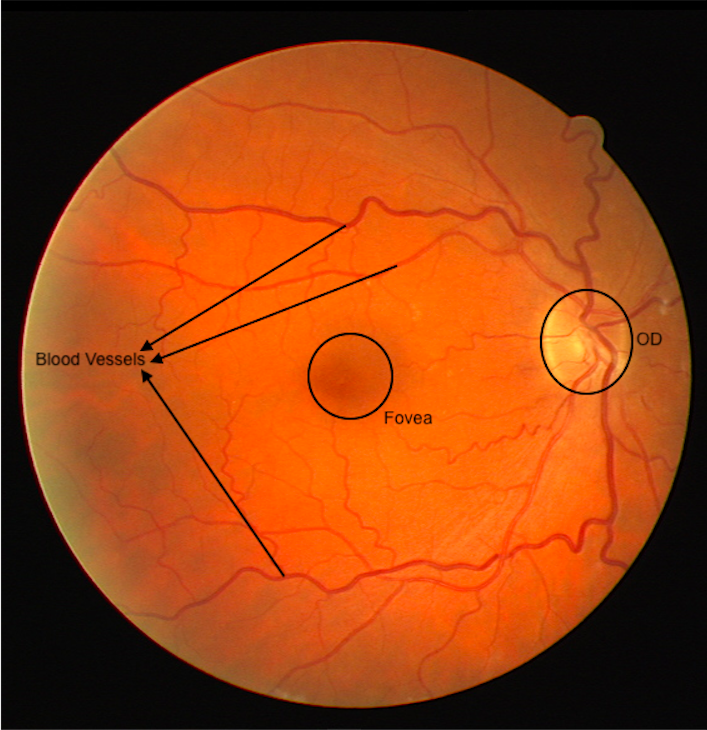
\includegraphics[width=\linewidth]{images/eye.png}
  \caption{Sample fundal image showing important structures}
  \Description{Sample fundal image showing important structures}
  \label{sample_funal_image}
\end{figure}

\begin{figure}[!ht]
  \centering
  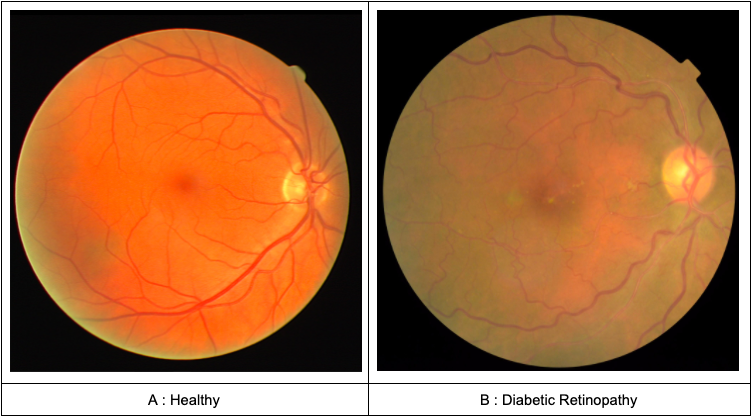
\includegraphics[width=\linewidth]{images/Comparison.png}
  \caption{Fundal image of healthy and diabetic retinopathy }
  \Description{Fundal image of healthy and diabetic retinopathy }
  \label{healthy_vs_dr}
\end{figure}

\section{Related Work}
Existing  techniques for blood vessel and Optic disc segmentation in fundal images mainly fall under two categories 1) using traditional image processing techniques and 2) using deep learning techniques.
Examples of image processing based techniques includes techniques using matched filters \cite{zhang2010retinal} \cite{hoover2000locating}, approaches using Gabor filters \cite{yavuz2011retinal} \cite{aslan2018segmentation} and techniques based on morphological operations \cite{hassan2015retinal}\cite{singh2014new} \cite{sumathy2012retinal}.
The image processing based techniques have the advantage that they don’t need the ground truth images annotated by human experts, but their performance is far behind the deep learning based approaches.
Further, these algorithms are based on many tunable thresholds that vary from dataset to dataset and they work based on some assumptions like gaussian distribution.

Several deep learning architectures that were found successful in segmentation tasks \cite{chen2017deeplab}\cite{long2015fully} in natural images were tried for segmenting blood vessels in retinal images and the results were significantly better than using conventional image processing techniques.
In \cite{vengalil2016customizing} a state-of-the-art segmentation model deeplab \cite{chen2017deeplab}, which is pre-trained on MSCOCO dataset \cite{lin2014microsoft}  for semantic segmentation,  was used to segment blood vessels at pixel level.
Jiang et.al. proposes \cite {jiang2018retinal} a  pre-trained fully convolutional network for segmenting blood vessels and report accuracy of cross-dataset test on four different datasets.
In M-GAN \cite{park2020m}, introduced by Kyeong et.al., a multi-kernel pooling block added between stacked convolutional layers supports scale-invariance which is a highly desirable feature for blood vessel segmentation.

One of the main challenges in using deep neural networks for segmentation tasks is that the reduction in resolution of featuremap as one goes deeper will result in loss of finer details like edges, which are crucial for segmentation tasks.
In order to circumvent this, the U-Net \cite{ronneberger2015u} model was introduced specifically for medical image segmentation which has multiple skip connections.
In their recent work, Joshua et.al. \cite{joshua2020blood} used a modified version of U-NET for segmenting blood vessels in retinal images and reported state of the art accuracies.
In Laddernet, introduced by Zhuang et.al. in 2018 \cite{zhuang2018laddernet},  is a sequence of multiple U-Nets cascaded together.

\section{Proposed Method}
We used a modified version of the UNET architecture for segmenting blood vessels and optic disc.
The network outputs a binary image, of the same resolution as the input,  which indicates pixel by pixel segmentation for blood vessels and/or optic disc.
For simultaneous prediction of optic disc and blood vessels, one additional channel is added at the output of the network resulting in a network with two output channels one for optic disc prediction and the other one for blood vessels prediction.

Figure \ref {unet_combined}  shows the architecture of the network used for simultaneous prediction.
The encoder and decoder consists of 4 stages each.
Each stage of the encoder comprises two convolution layers, each followed by batch normalization and ReLU activation function.
A max-pooling layer with a stride of 2 is added at the end of each stage of the encoder which down samples the image by a factor of two.
Each decoder layer up-samples the image by a factor of 2 using  a deconvolution layer followed by a convolution layer.

\begin{figure}[!ht]
  \centering
  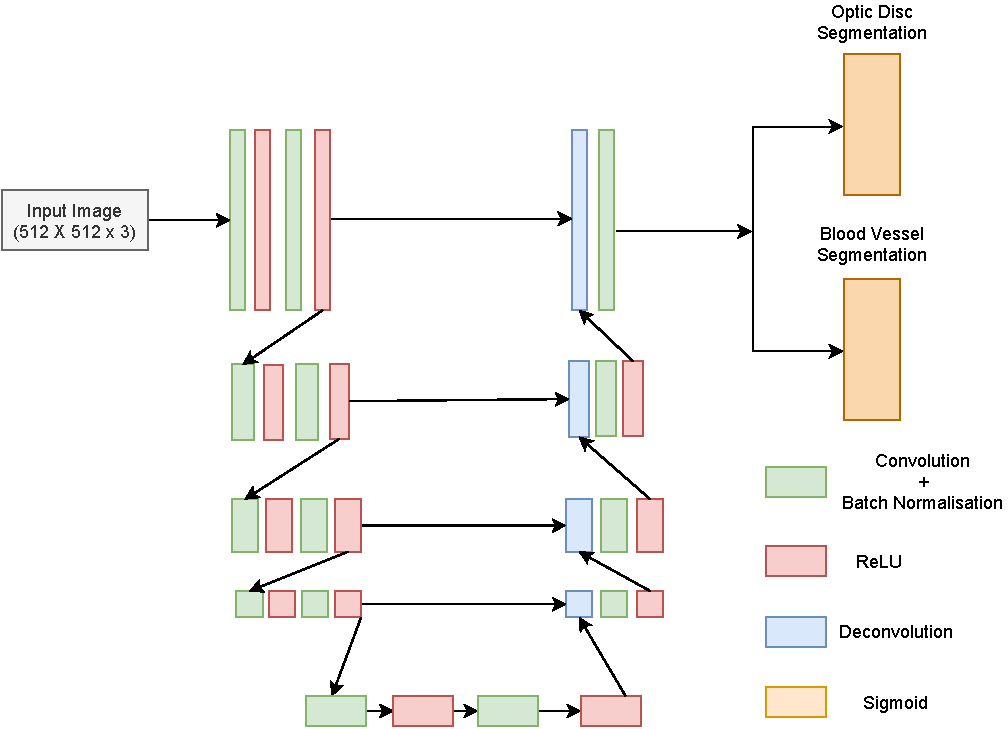
\includegraphics[width=\linewidth]{images/UnetArch.pdf}
  \caption{Fundal image of healthy and diabetic retinopathy}
  \Description{Fundal image of healthy and diabetic retinopathy}
  \label{unet_combined}
\end{figure}

\subsection{Dataset}
We used the DRIVE \cite{drive} and HRF \cite{budai2013robust}  datasets for blood vessel segmentation and optic disc segmentation.
The DRIVE dataset contains 20 training images and 20 testing images of resolution $565 \times 584$ pixels.
The dataset also provides ground truth images for blood vessel segmentation annotated by a human expert.
As the DRIVE dataset does not have optic disc annotations, we annotated the optic disc in each image ourselves.
HRF dataset has 15 high resolution fundal images along with ground truth annotation for blood vessel segmentation.
We used 10 images for training and  remaining 5 images  were used for evaluation.

Unlike many other existing methods where image patches are used to train a  deep learning model in order to increase the training set, we used full images for training our combined prediction network as a full image will have more context and hence can be more effective for predicting structures like optic disc.
We used data-augmentation, provided by the library Albumentations \cite{buslaev2020albumentations}, in order to generate more training images as required by typical deep learning models.
From each image 4 different images were generated using the following data augmentations.
\begin{enumerate}
  \item Horizontal flipping
  \item Vertical flipping
  \item Elastic transform
  \item Grid Distortion
\end{enumerate}
A sample of each of the above data augmentation, when applied on DRIVE images,  is shown in Figure \ref{data_augmentation}.

\begin{figure}[!ht]
  \centering
  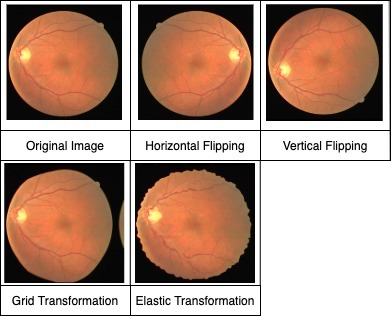
\includegraphics[width=\linewidth]{images/Data_Augmentation.jpg}
  \caption{Sample images for each data augmentation. Note that even though the images created by elastic and grid distortion do not look like a real fundal image, they can help to reduce overfitting.}
  \Description{Sample images for each data augmentation}
  \label{data_augmentation}
\end{figure}

\subsection{Loss function and training}
A softmax activation function is used at the output layer which predicts the probability of each pixel being a blood vessel (or optic disc for the second output channel).
The model is trained with weighted binary cross entropy loss and adam optimizer.
For predicting optic disc and blood vessel separately,  two separate networks with the same architecture are trained independently using loss function given below in equation \ref{loss_od} and \ref{loss_bv} respectively.

\begin{equation}\label{loss_od}
L_{OD} = -\sum_{i,j} y_{ij}^{OD}log(\hat{y}_{ij}^{OD} ) - \alpha_{OD}(1-y_{ij}^{OD} )log(1-\hat{y}_{ij}^{OD})
\end{equation}

\begin{equation}\label{loss_bv}
L_{BV} = -\sum_{i,j} y_{ij}^{BV}.log(\hat{y}_{ij}^{BV}) - \alpha_{BV}(1-y_{ij}^{BV})log(1-\hat{y}_{ij}^{BV})
\end{equation}

Where the summation is over all the pixels in the image, $y_{ij}^OD$ is the true optic disc label and  $\hat{y}_{ij}^OD$ is the predicted optic disc label.
Similarly, $y_{ij}^{BV}$ and $\hat{y}_{ij}^{BV}$ are the true and predicted blood vessel labels.
$\alpha_{OD}$ and $\alpha_{BV}$ are the class weights for optic disc and blood vessel respectively.

When trained separately, the networks are not able to take advantage of the correlation between the two tasks.
In the multi-tasking model, we used a single network with two output channels as shown in Figure \ref{unet_combined} and the losses given in equation \ref{loss_od} and \ref{loss_bv} above are computed at channel 1 and channel 2 respectively.
The final loss function for multi-tasking model is obtained by adding the two losses together as given in equation \ref{loss_multi-tasking} below

\begin{equation}\label{loss_multi-tasking}
  L = L_{OD} + L_{BV}
\end{equation}

The network was trained for 60 epochs in the both the cases.

\begin{figure}[!ht]
  \centering
  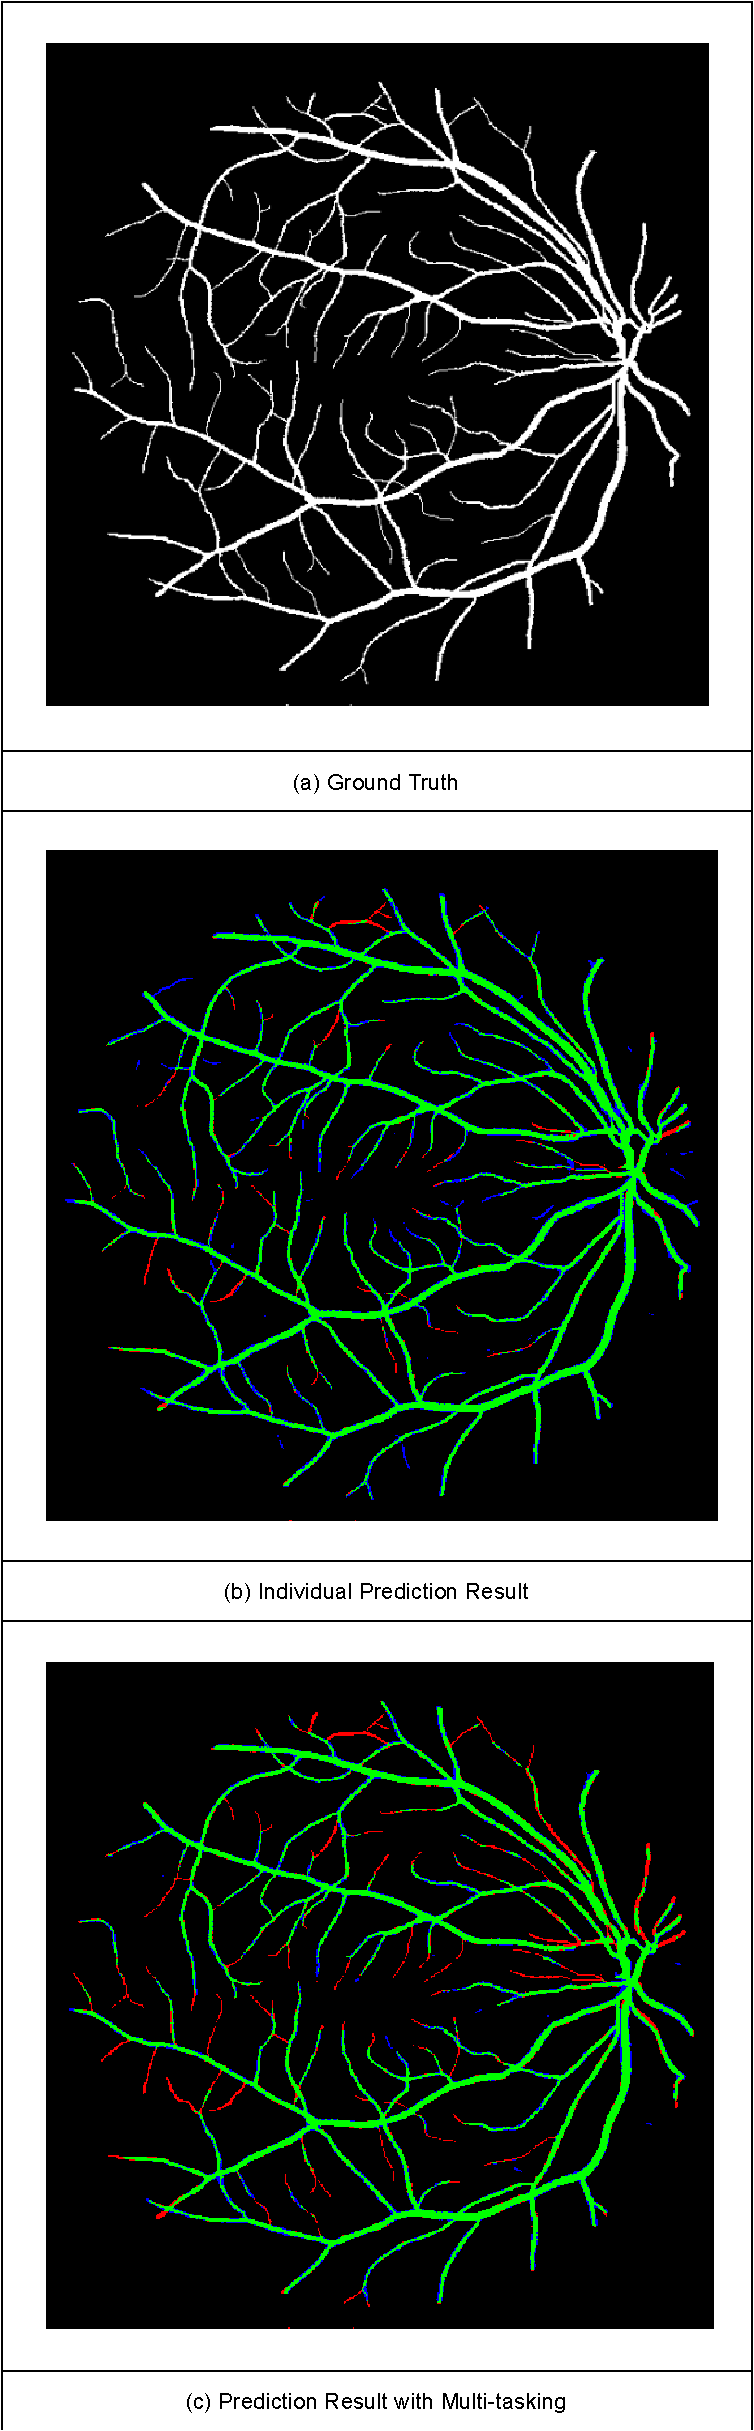
\includegraphics[width=0.6\linewidth]{images/Prediction_Results (1).pdf}
  \caption{Comparison of  blood vessel prediction for drive test image. a) Ground truth b) using individually trained model c) using multi-tasking model }
  \Description{Comparison of result of Blood vessel prediction  performed individually and  blood vessel and optic disc combined}
  \label{simultaneous_vs_individual}
\end{figure}

\section{Results and Discussion}
Figure \ref{simultaneous_vs_individual} shows a comparison of  simultaneous prediction of blood vessel and optic disc on DRIVE  datasets with that of individual prediction using separate networks.

The average F1-score on all DRIVE test images was 0.78 with multi-tasking whereas without multi-tasking the F1 score was 0.72.
From Figure \ref{simultaneous_vs_individual}, it is seen that even though the recall reduces with multi-tasking (more number of missed predictions shown in red pixel in the figure), precision improves significantly (less number of false positives- blue pixels in the figure).
The significant increase in precision with multi-tasking results in an overall improvement in F1 score.

For optic disc segmentation with multi-tasking, the F1 score was increased from 0.72 without multi-tasking to 0.76 with multi-tasking.

We also performed experiments on HRF dataset and got an F1 score of 0.79 with multi-tasking for blood vessel segmentation.
Without multi-tasking, the F1 score on HRF dataset was 0.78 for blood vessel segmentation.

The improved performance in both the cases are a consequence of direct correlation between the distribution of blood vessels and the optic disc in the retinal image.
When trained together, the network is able to learn new hidden layer features that can contribute to the prediction of both blood vessels and optic disc.

\section{Conclusion}
In this work, we evaluate the effectiveness of multi-tasking deep learning models for segmenting blood vessels and optic disc in fundal images.
We build a multi-tasking model, and corresponding loss function,  based on the famous U-Net architecture for simultaneous  segmentation of blood vessels and optic disc.
Our results show an increase in F1 score from 0.72, without multi-tasking, to 0.78 with multi-tasking for blood vessel segmentation.
Similarly for optic disc the F1 score was lifted to 0.76 with multi-tasking from 0.72 without multi-tasking.
On HRF dataset we got an F1 score of 0.79 with multi-tasking and 0.78 without multi-tasking for blood vessel segmentation.
In addition to the performance improvement in F1 score, the training and prediction time is also reduced by almost half as the weights of the network until the last layer remains same for both optic disc and blood vessel prediction.